\begin{enumerate}
	\item \begin{enumerate}
		      \item Solutions that start with $-1<y<2$ have an $s$-curve shape sloping down. Solutions
		            that start with $y>2$ look like exponentials. Solutions that start with $y< -1$ look like
		            negative exponentials (i.e. $\exp(-t)$). And solutions that start with $y=2$ or $y=-1$ are
		            constant functions.
		      \item No. Using the equation we see $y'(0)=-2\neq 0$. Further, we can see from the slope
		            field that a solution starting at $y=0$  will not be constant.
		      \item Computing, $f'(y) = 2y-1$, and so $f'(0)=-1$. Thus,
		            \[
			            A_0(y) = -(y-0) -2=-y-2.
		            \]
		      \item \phantom{.}

		            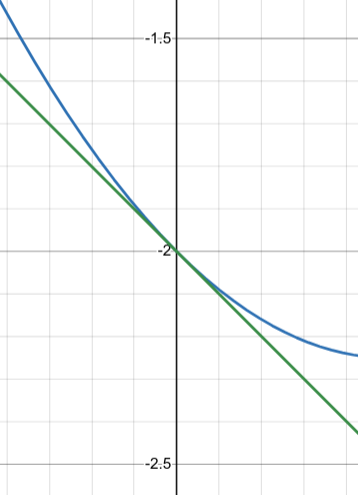
\includegraphics[width=2in]{./resources/tutorial-07-1d.png}

		            It looks like $A_0$ is a good approximation when $-0.12\leq y\leq 0.12$.

		      \item The general solution to $y'=-y-2$ is $y(t)=Ae^{-t}-2$. To find $A$ we plug in our initial
		            condition to get
		            \[
			            y_{\text{approx}}(t)=2e^{-t}-2.
		            \]

		      \item $y_{\text{approx}}$ should be a good approximation of the solution to Equation (A) as long as
		            $-0.12 \leq y_{\text{approx}}(t)\leq 0.12$. By using the formula for $y_{\text{approx}}$,
		            we find this is when $-0.058\leq t \leq 0.06$.
		      \item In the figure below, you can see the solution to Equation (A) in solid blue and $y_{\text{approx}}$ in dashed orange.

		            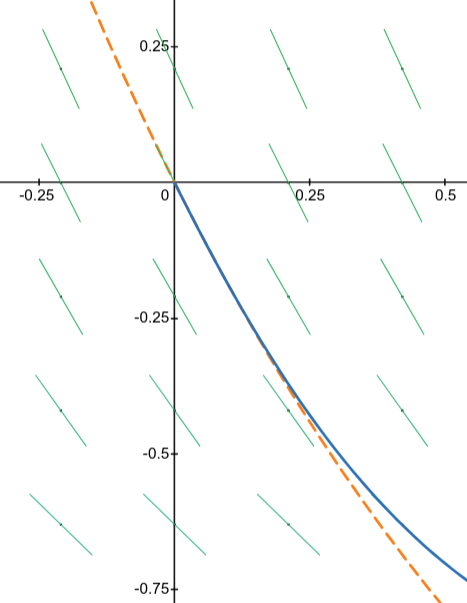
\includegraphics[width=2in]{./resources/tutorial-07-1g.png}

		            It looks like $y_{\text{approx}}$ stops being a good approximation around $t=0.18$, which means
		            that it is a much better approximation than we expected.

		      \item The equilibrium solutions are $y=-1$ and $y=2$.

		            \textbf{Case $y=-1$:}

		            We have an approximation $A_{-1}(y) = -3y-3$. The differential equation $y'=A_{-1}(y)=-3y-3$ has
		            an \emph{attracting} and \emph{stable} equilibrium solution $y=-1$, and so the equilibrium solution
		            for Equation (A) at $y=-1$ is \emph{attracting} and \emph{stable}.

		            \textbf{Case $y=2$:}

		            We have an approximation $A_{2}(y) = 3y-6$. The differential equation $y'=A_{2}(y)=3y-6$ has
		            a \emph{repelling} and \emph{unstable} equilibrium solution $y=2$, and so the equilibrium solution
		            for Equation (A) at $y=2$ is \emph{repelling} and \emph{unstable}.
	      \end{enumerate}
	\item \begin{enumerate}
		      \item Equation (B) cannot be written in matrix or affine form.
		      \item
		      \item The equilibrium solution at $\mat{-1\\1}$ appears to be attracting.
		      \item The total derivative of $\vec F$ at $\mat{-1\\1}$ can be expressed by the matrix
		            \[
			            \mat{-1&0\\-2&-1}.
		            \]
		      \item \[
			            \vec A(x,y) = \mat{-1&0\\-2&-1}\left(\mat{x\\y}-\mat{-1\\1}\right)
		            \]
		      \item We see the eigenvalue of $\mat{-1&0\\-2&-1}$ is $-1$ with geometric and algebraic multiplicity $2$.
		            Therefore its unique equilibrium solution is \emph{stable} and \emph{attracting}.
		      \item Since $\vec A$ is an affine approximation to $\vec F$ at $\mat{-1\\1}$, we know the nature
		            of the equilibrium solution at $\mat{-1\\1}$ should be the same for both $\vec r\,'=\vec F(\vec r)$
		            and $\vec r\,'=\vec A(\vec r)$ (provided that the real part of each eigenvalue is non-zero).
		            Since $\vec r\,'=\vec A(\vec r)$ has a stable and attracting equilibrium solution at $\mat{-1\\1}$,
		            so does $\vec r\,'=\vec F(\vec r)$.

		      \item The remaining equilibrium solutions are $\vec r(t)=\mat{\sqrt{2}\\2}$ and $\vec r(t)=\mat{-\sqrt{2}\\2}$.
		            After linearizing at $\mat{\sqrt{2}\\2}$ and $\mat{-\sqrt{2}\\2}$, we find that both equilibrium solutions
		            are \emph{unstable} but not \emph{repelling} (the corresponding matrices have a mix of one positive and one negative eigenvalue).

	      \end{enumerate}
\end{enumerate}